\chapter{Final Design} \label{chapter:final-design}
The last usability study has shown that the interface still has two major problem areas: the diff view and the saving process. In this chapter solutions for these problems are proposed as well as fixes for the smaller usability issues discovered during the previous study.

\section{Difference View}
The most severe and impactful usability issues occurred in connection with the diff view during the last study. The main problem was that the representation of content in the diff view was very fragmented and fundamentally different from the way content was represented to the user when editing it (Issues \#37 and \#38). Furthermore, some users did not understand how to use the breadcrumb navigation in order to jump back and forth between the list of changes and the actual editing view (Issue \#39). For some users, it was not even clear which part of the diff showed the old and which part the new state (Issue \#40).

In order to eliminate these issues a new design for the diff view was developed (Figure \ref{fig:diff-split}). The new layout shows two tables next to each other, that are more or less identical to the ones in the editing view, except that they are read-only and cannot be edited. The old state of the content is shown in the table on the left and the changes are marked in red. The new state is shown on the right-hand side and changes are marked in green. The view only displays those rows that have been edited, the remaining ones are hidden by default, but can be shown by clicking on the button at the bottom. Content that has not changed is somewhat transparent to visually lay more focus on the edited content.

Using the same representation as in the editing view makes recognizing the structure of the content a lot easier. Jumping between diff view and editing view only to get a feeling of the structure of the content is no longer necessary. By this, the most problematic parts of the old design are removed and the mental effort to review changes should be smaller now.


% closer to editing representation
% analogy: code is represented in the diff as it is edited -> same should be true for language content

\begin{figure}[h!]
 \centering
 \fbox{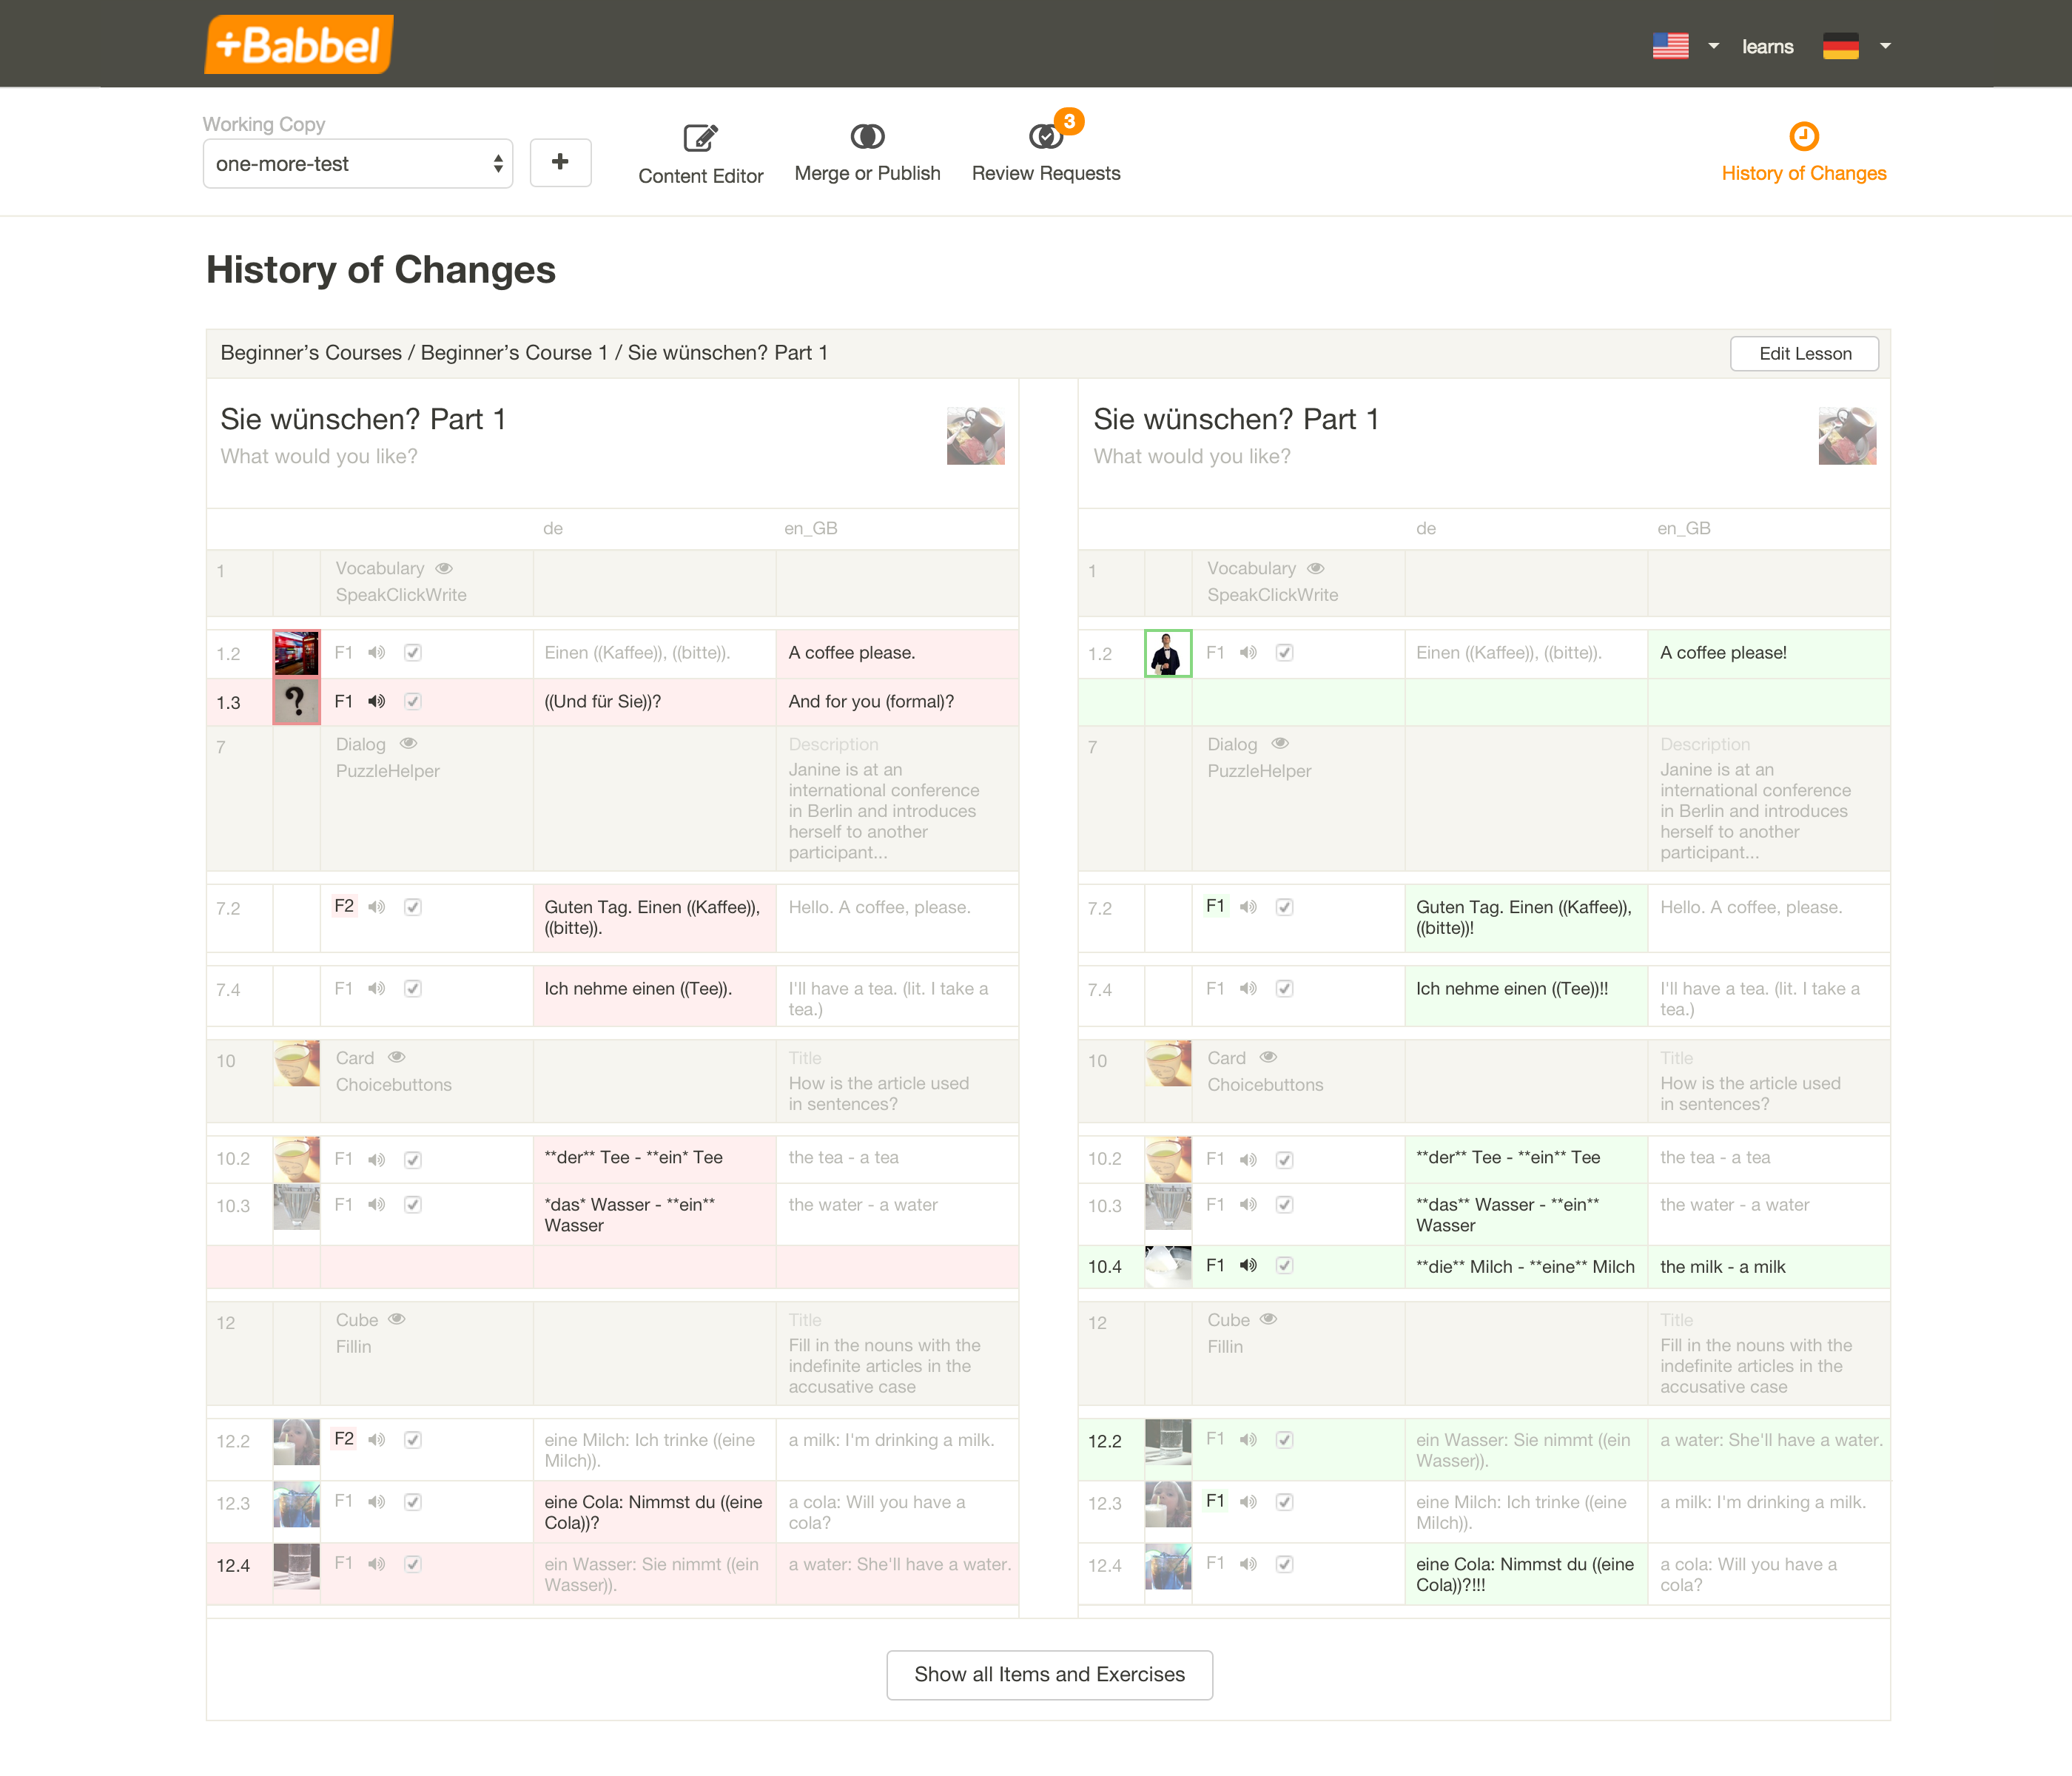
\includegraphics[width=\textwidth]{final-design/diff-split}}
 \caption{New difference view}
 \label{fig:diff-split}
\end{figure}
% this figure needs to be changed (nav bar is old)

\section{Saving Process}
Saving changes was one of the major pitfalls for users during the last usability study. The redesigned saving process addresses the issues \#41 and \#43 listed in Table \ref{table:issues-saving}. Most of all, users were confused by the existence of two separate saving features (Issue \#41). Even though the saving "shortcut" at the bottom of the editing view was used frequently, it caused confusion when users discovered there is also a second saving button at the top. For this reason, the two separate saving features were combined into one by trying to maintain the advantages of both. The new saving process (Figure \ref{fig:highlighted-changes}) allows users to save their changes on the same page as the edits were done while at the same time giving them the opportunity to review what has changed. The changes are highlighted in green and when hovered reveal the state prior to editing it. Users can decide whether they want to enable this highlighting by toggling a checkbox at the bottom of the view.

Additionally to reducing the steps required to save changes, the new feature also provides better feedback (Issue \#43), because the highlighting disappears after the user saved, signalling that there are no current changes that were not saved yet.

% using two separate saving features wasn't practical. during the user tests it became clear that a global saving function is not needed. whereas in programming it is often necessary to edit several files in order to implement a certain feature in language authroing the editing context is always defined by the immediate surroundings.


\begin{figure}[h!]
 \centering
 \fbox{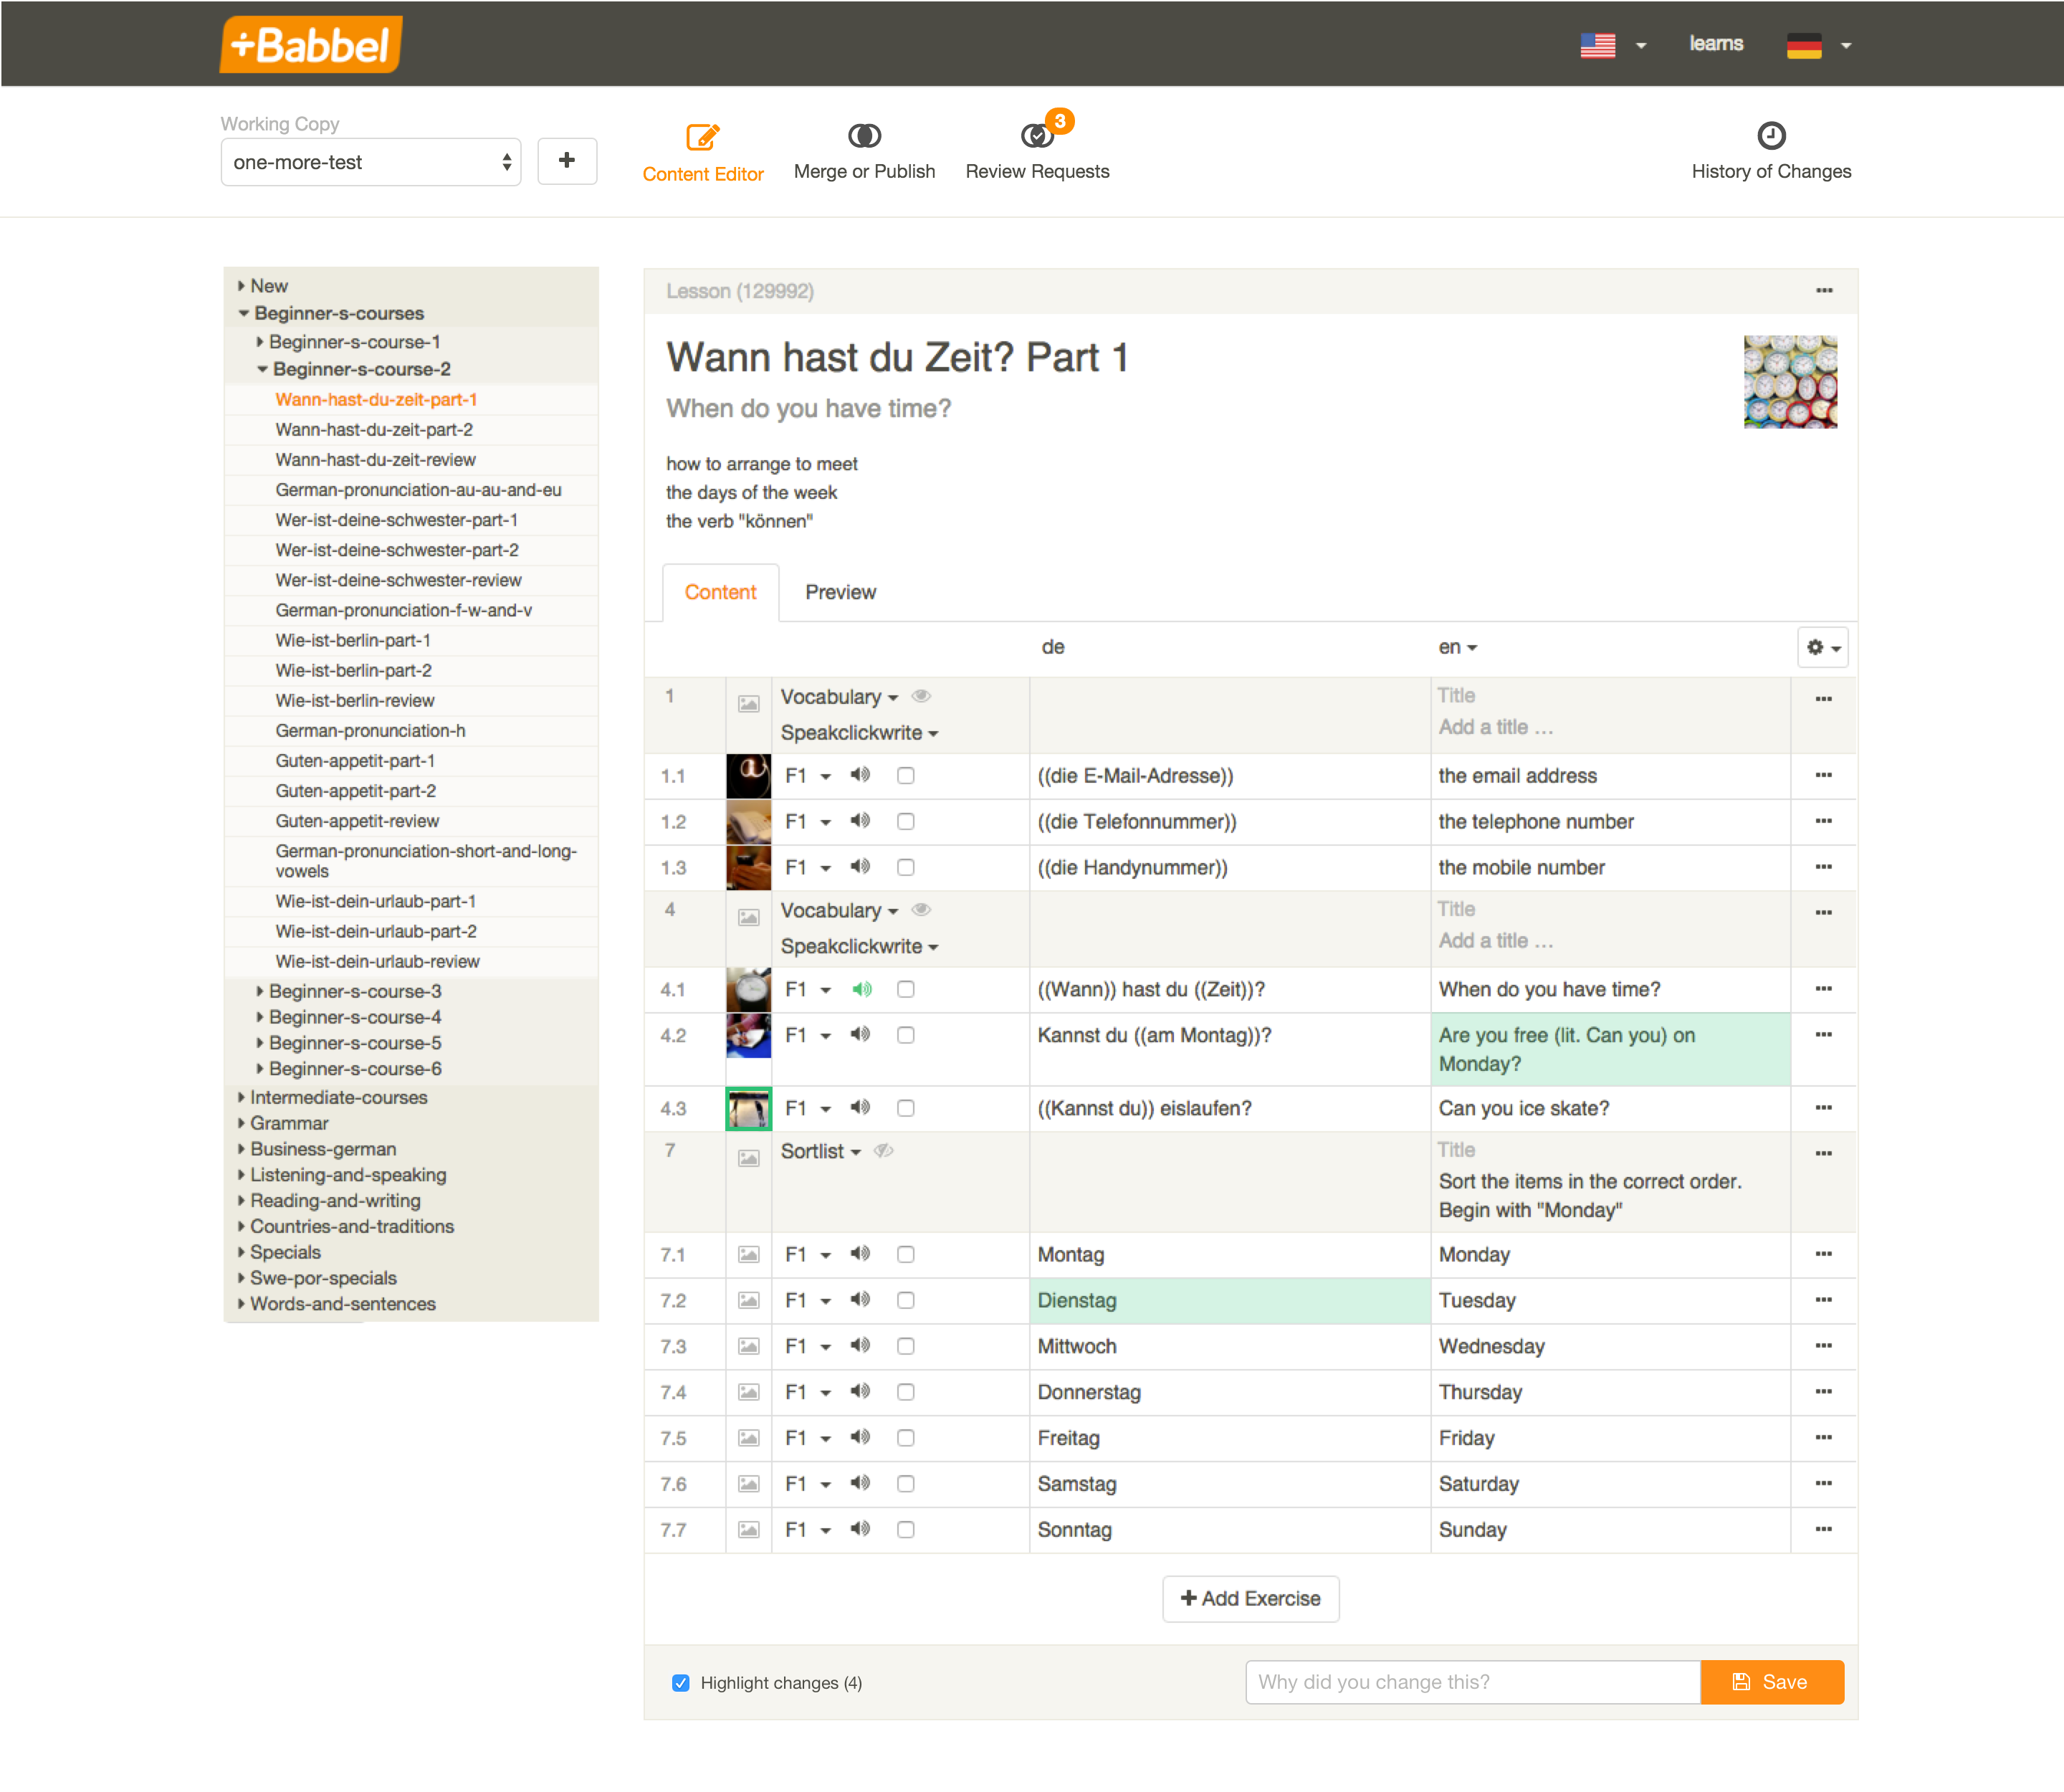
\includegraphics[width=\textwidth]{final-design/edited-highlighting}}
 \caption{Highlighted changes after editing}
 \label{fig:highlighted-changes}
\end{figure}

\begin{figure}[h!]
 \centering
 \fbox{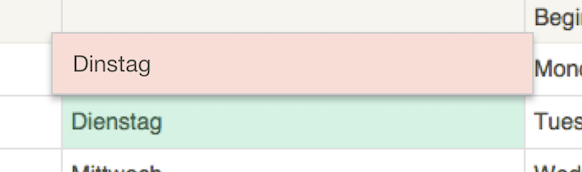
\includegraphics[width=4cm]{final-design/saving-hover-text}}
 \caption{Hovering a changed text}
 \label{fig:hover-changed-text}
\end{figure}

\begin{figure}[h!]
 \centering
 \fbox{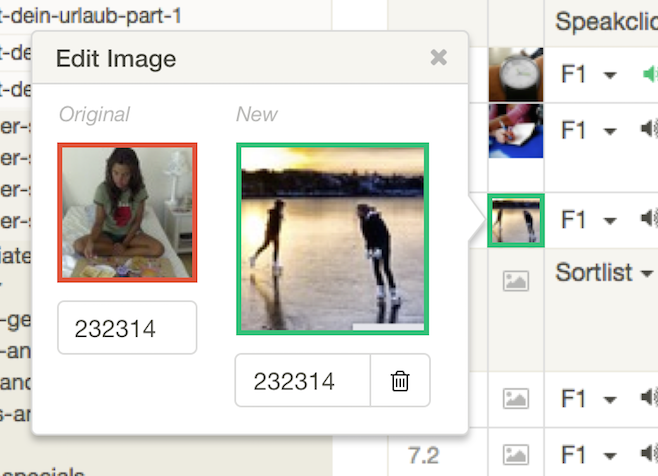
\includegraphics[width=4cm]{final-design/saving-hover-image}}
 \caption{Hovering a changed image}
 \label{fig:hover-changed-image}
\end{figure}


\section{Error Messages}
Another problem that occurred quite frequently during the previous testing sessions were missing or insufficient error messages. Especially during the creation of new working copies, users got stuck, because the interface did not provide appropriate information for recovering from a mistake. The two most common problems where using invalid characters or trying to use a name that was already taken. Now, there are error messages informing users about this (Figure \ref{fig:improv-error-messages}).

Furthermore, the system is more pro-active now. Even though it is technically possible to create an empty merge request, in reality there is no value in doing that. Therefore, the interface now informs users when they are about to do it (Figure \ref{fig:empty-merge-warning}).

\begin{figure}[h!]
 \centering
 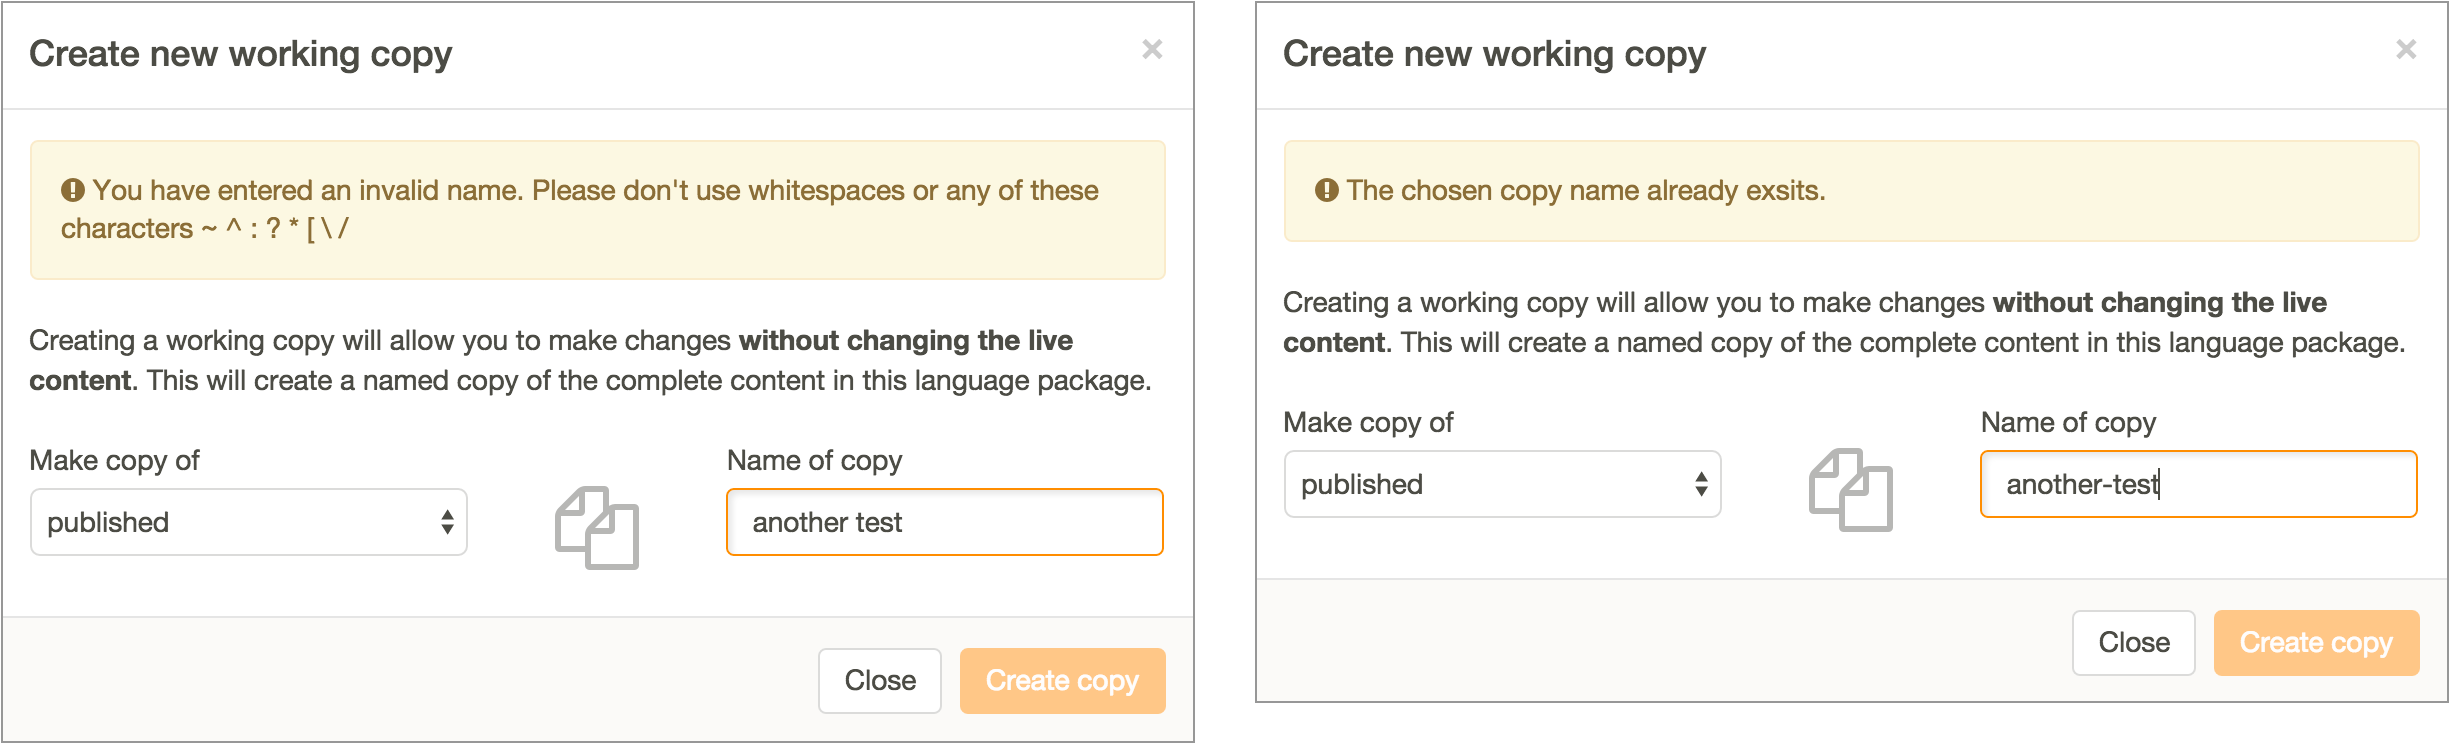
\includegraphics[width=\textwidth]{final-design/error-messages-modal}
 \caption{Improved error message inside working copy modal}
 \label{fig:improv-error-messages}
\end{figure}

\begin{figure}[h!]
 \centering
 \fbox{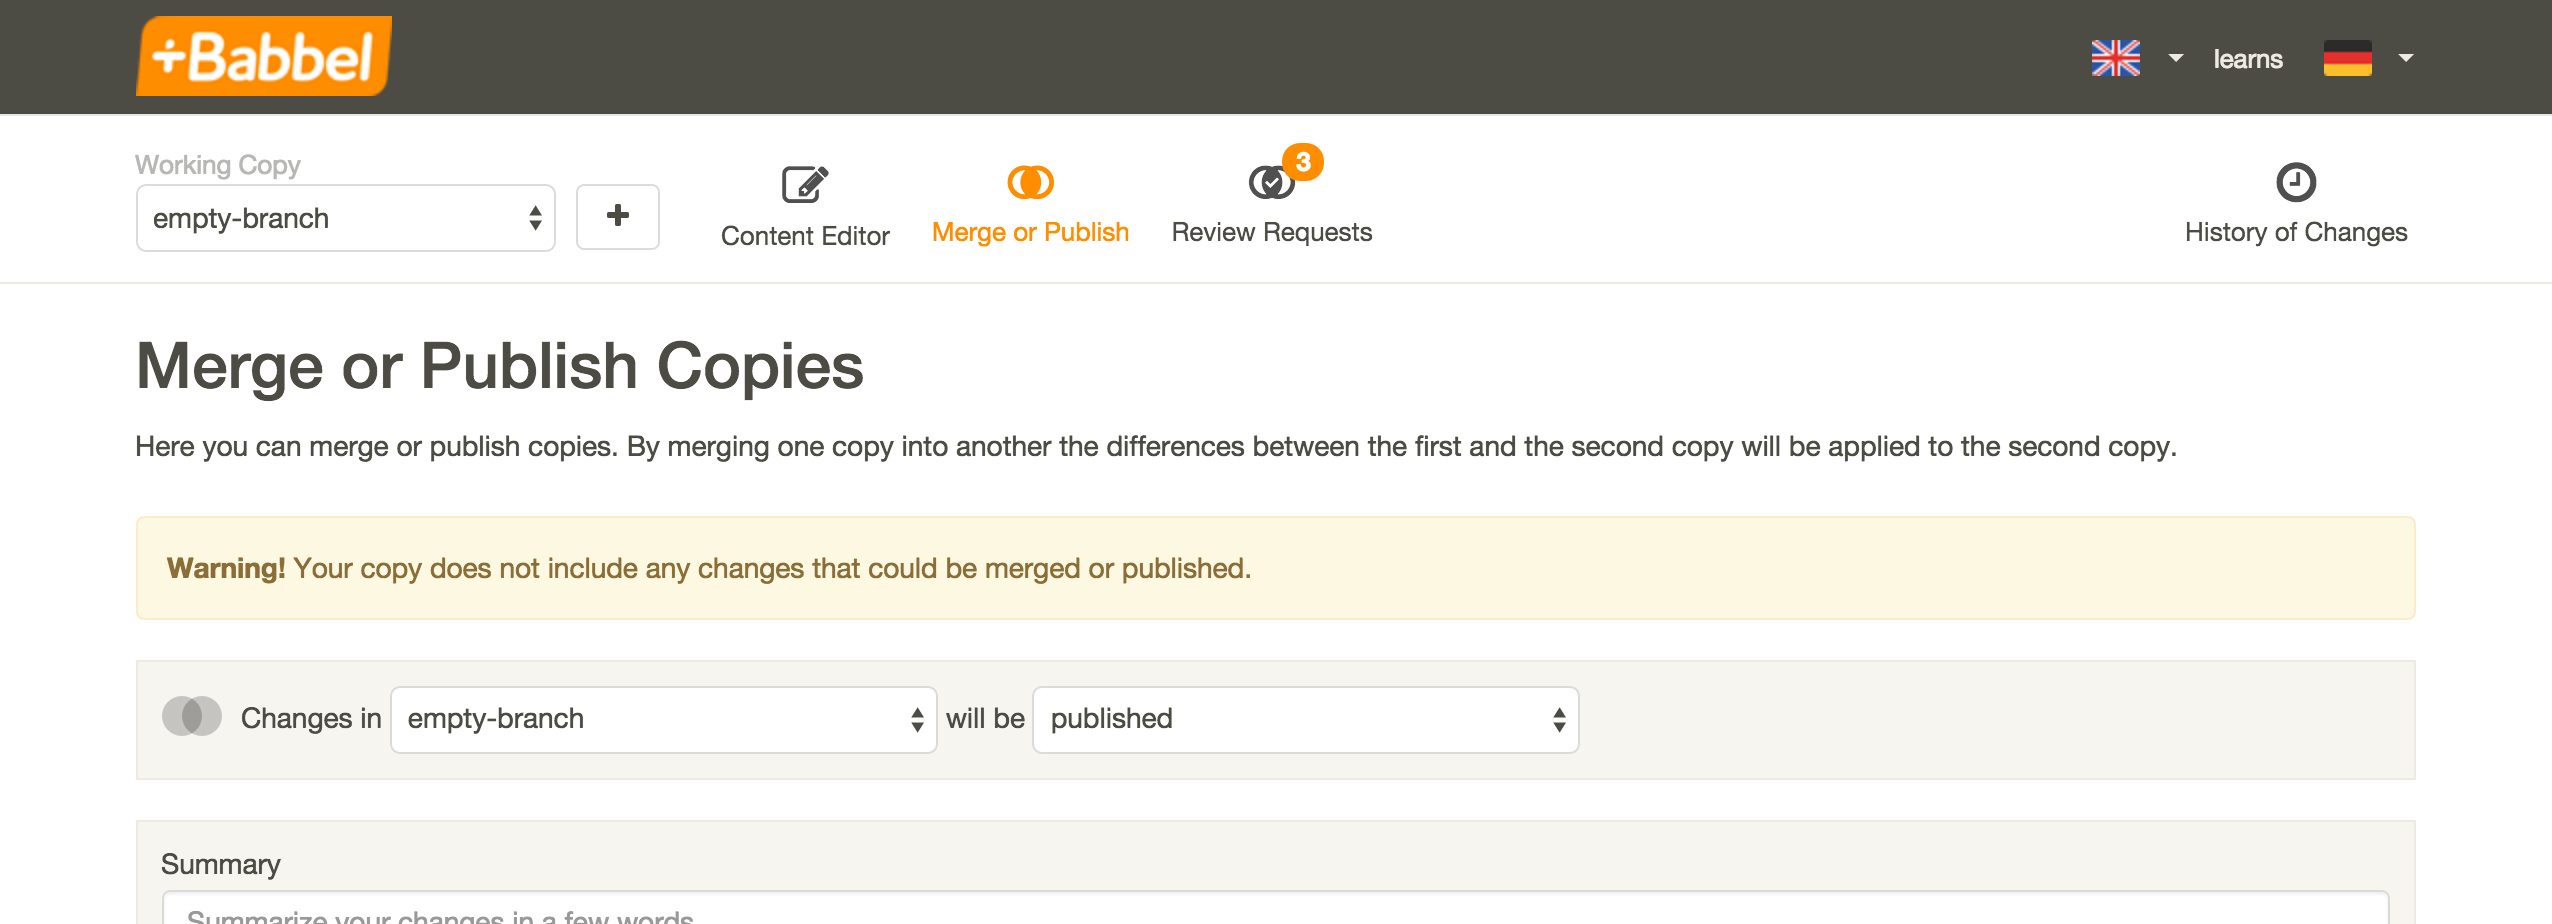
\includegraphics[width=\textwidth]{final-design/empty-merge-warning}}
 \caption{A warning informing users that the selected working copy is equal to the target of the merge}
 \label{fig:empty-merge-warning}
\end{figure}

\section{Navigation Bar}
The top-level navigation was changed conceptually, which also had to be reflected in the layout of the navigation bar (Figure \ref{fig:redesigned-nav}). Instead of treating the different views as "layovers", which were closed with a little \textit{x} in the upper right corner, the navigation now works more like a classical tab-style navigation. Therefore, a new icon for the content editor had to be introduced, which is now placed next to the working copy selection. The "new copy" button was visually grouped with the selection, because these two features conceptually belong together and because it triggered a different behaviour (opening a popup) then the remaining buttons, which result in a complete a view change.

\begin{figure}[h!]
 \centering
 \fbox{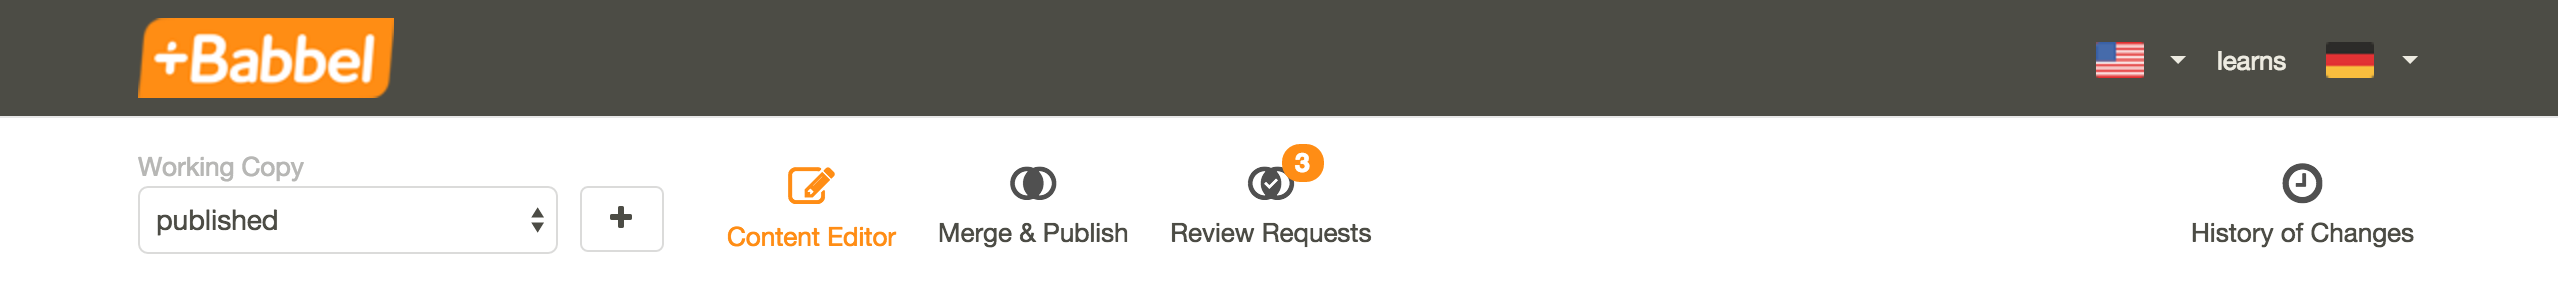
\includegraphics[width=\textwidth]{final-design/new-navigation}}
 \caption{Redesigned navigation bar}
 \label{fig:redesigned-nav}
\end{figure}

\section{Miscellaneous Changes}
In order to make the new diff view work, the lesson editing view had to be revised as well. So far, the lesson properties, which include the title, subtitle and a description for every display language, were hidden behind the properties tab. This design was impractical for the new diff view, because everything related to a lesson should be reviewable with just one glance. Therefore, the lesson properties were moved into the header of the editing view and editing was made possible by an inline-editing\footnote{http://ui-patterns.com/patterns/InplaceEditor} solution (Figure \ref{fig:new-lesson-header}). This means that the text turns into an input field when clicked and can be edited.

\begin{figure}[h!]
 \centering
 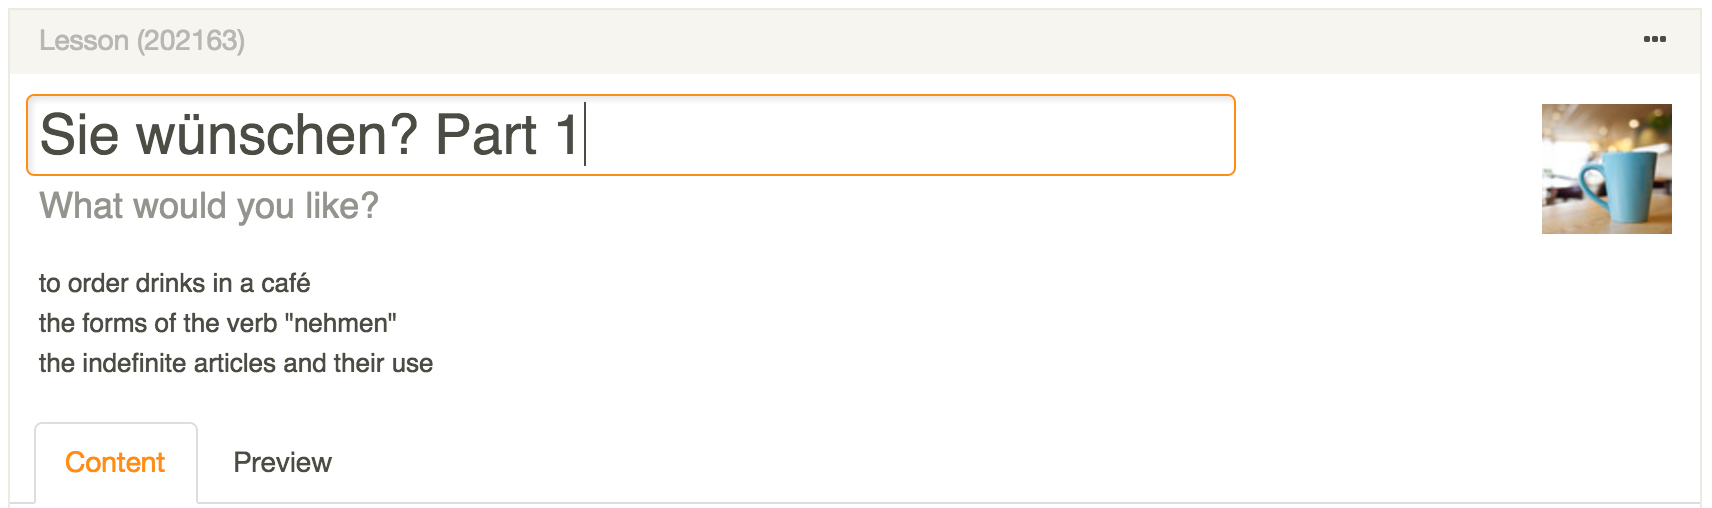
\includegraphics[width=9cm]{final-design/new-lesson-header-editing}
 \caption{New lesson header}
 \label{fig:new-lesson-header}
\end{figure}

The new lesson header design described above required another redesign. Now that changing the display language not only affected content that is inside the translation column, but also the text in the lesson header, it seemed odd to select this language in the table header as before. For this reason, the selection was moved to the main navigation bar at the top (Figure \ref{fig:dl-selection}) next to the selection of the learning language.

\begin{figure}[h!]
 \centering
 
\includegraphics[width=4cm]{final-design/dl-selection}
 \caption{Display language selection}
 \label{fig:dl-selection}
\end{figure}

Besides the conceptual changes and those that addressed usability issues directly, a few visual improvements were made in order to reduce the visual clutter. The form for merging or publishing copies was simplified and the input field for the second reviewer is now hidden by default (Figure \ref{fig:merge-publish}). Furthermore, the list of requests (Figure \ref{fig:review-requests}) and the list of changes (Figure \ref{fig:history-of-changes}) were simplified by removing the "show details" button and instead making the whole row clickable.

\begin{figure}[h!]
 \centering
 \fbox{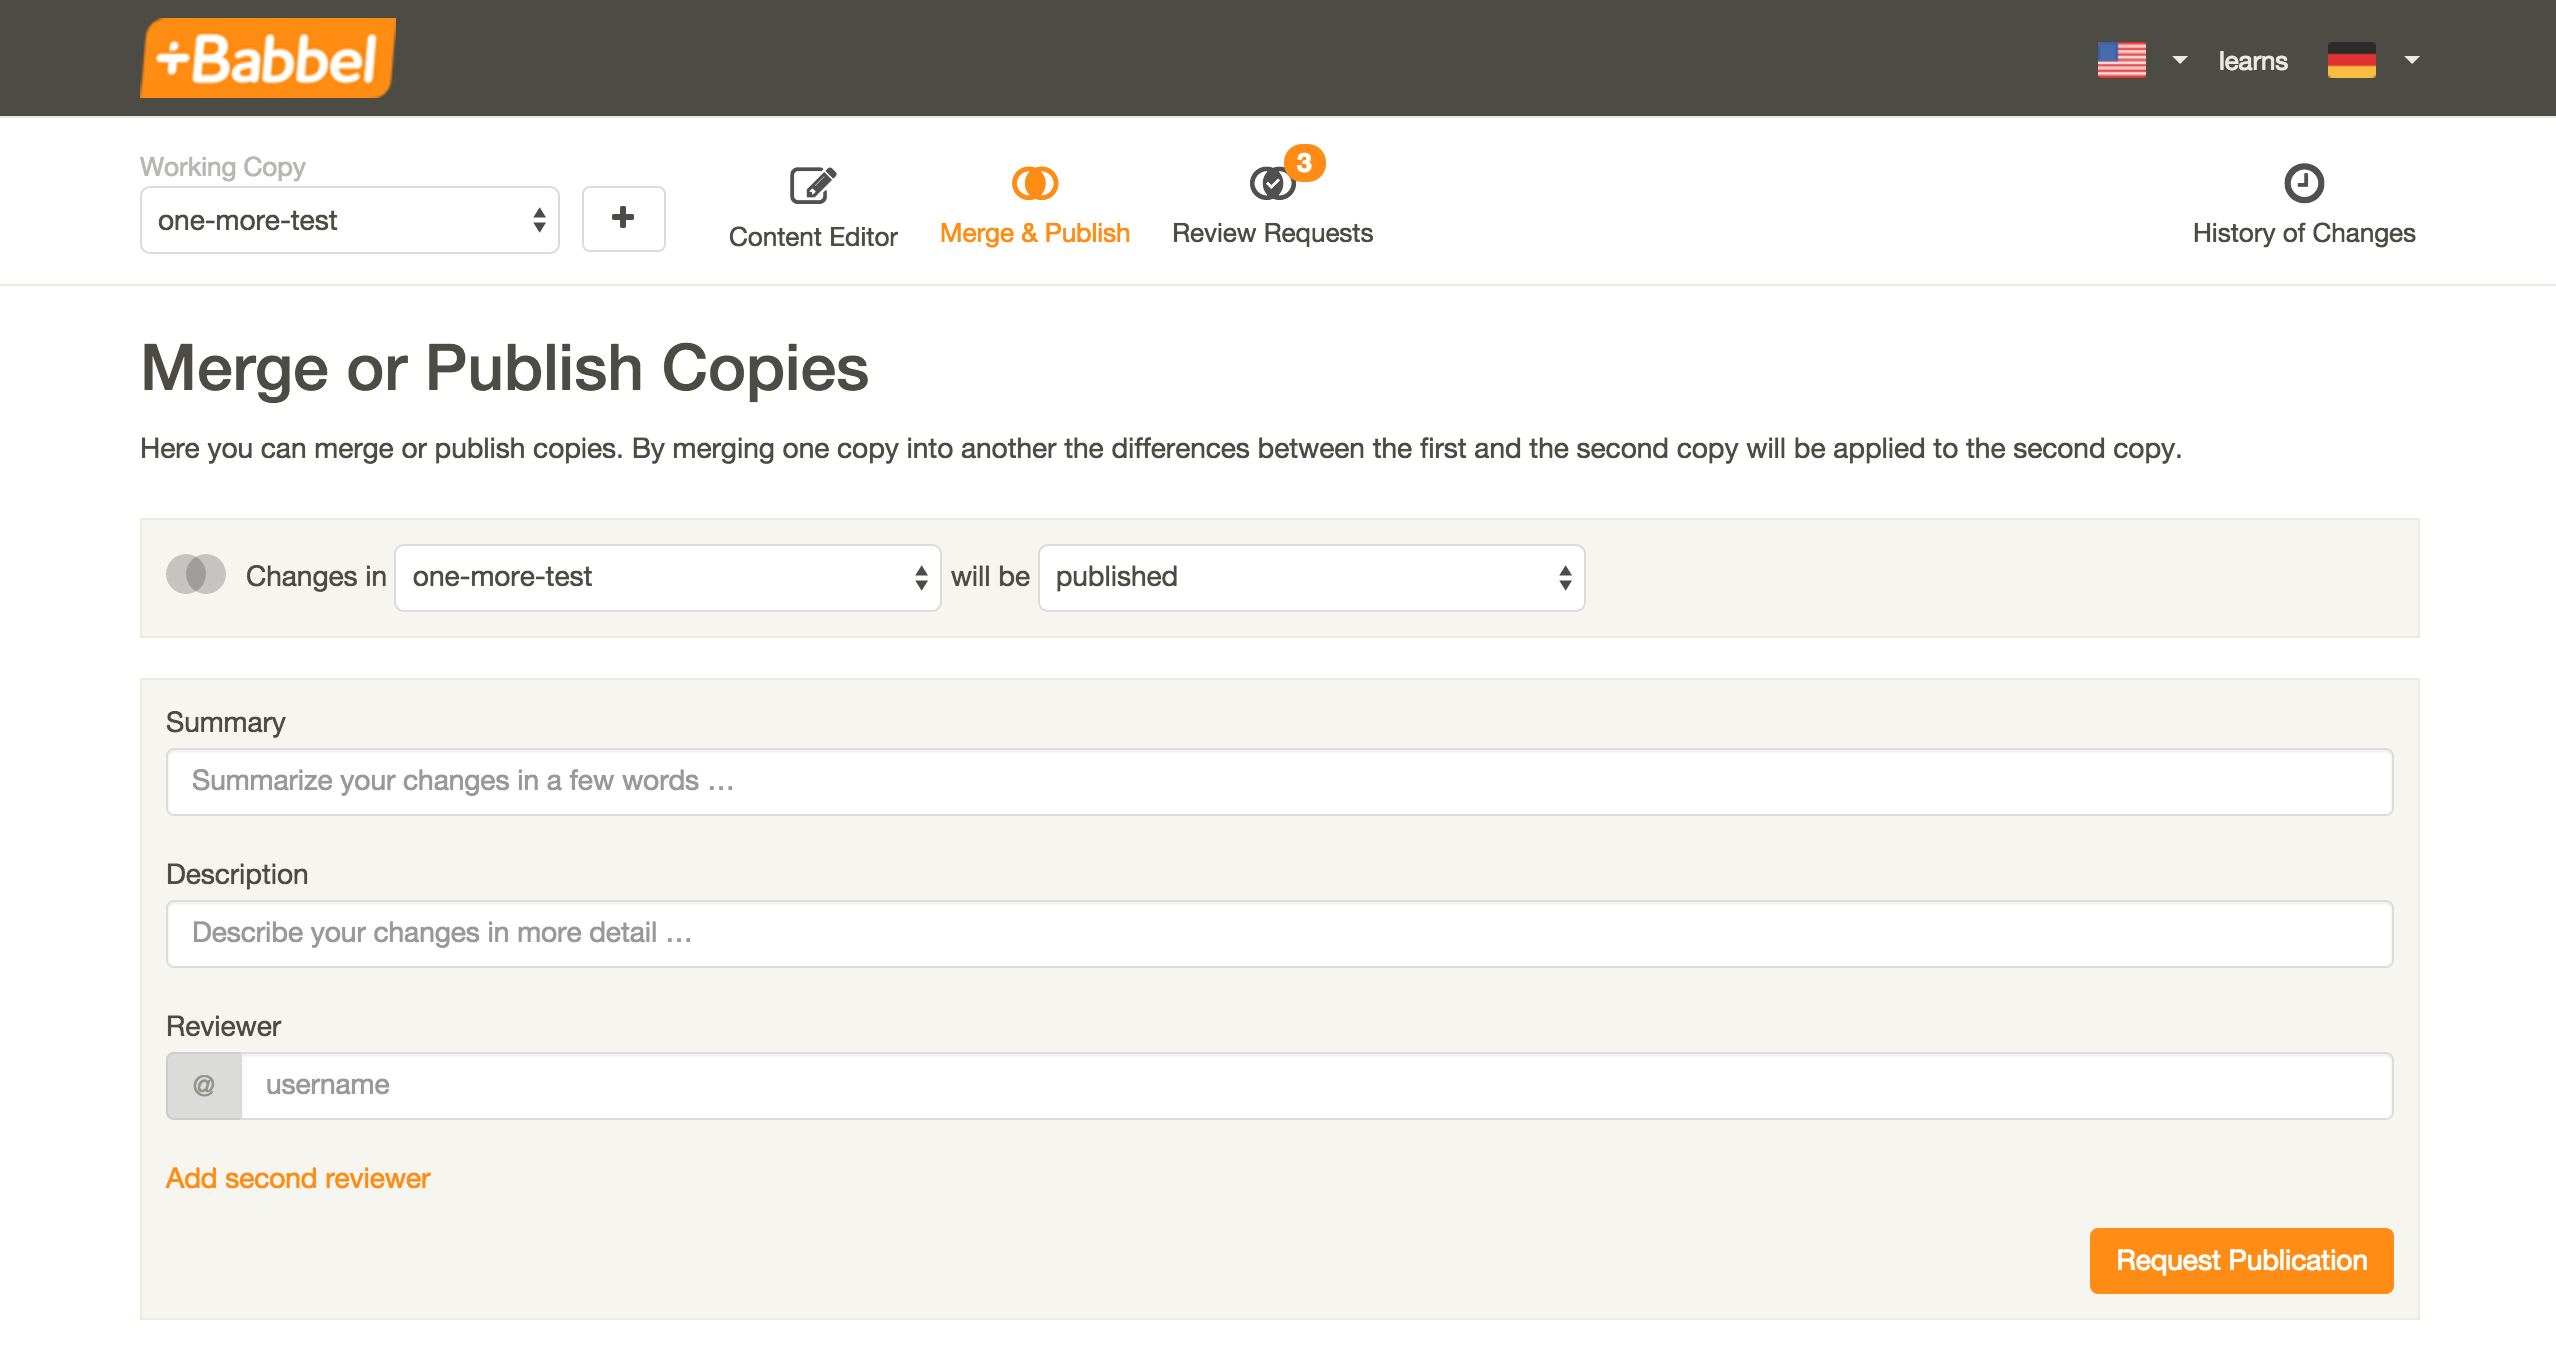
\includegraphics[width=\textwidth]{final-design/merge-or-publish}}
 \caption{Merge or publish copies}
 \label{fig:merge-publish}
\end{figure}

\begin{figure}[h!]
 \centering
 \fbox{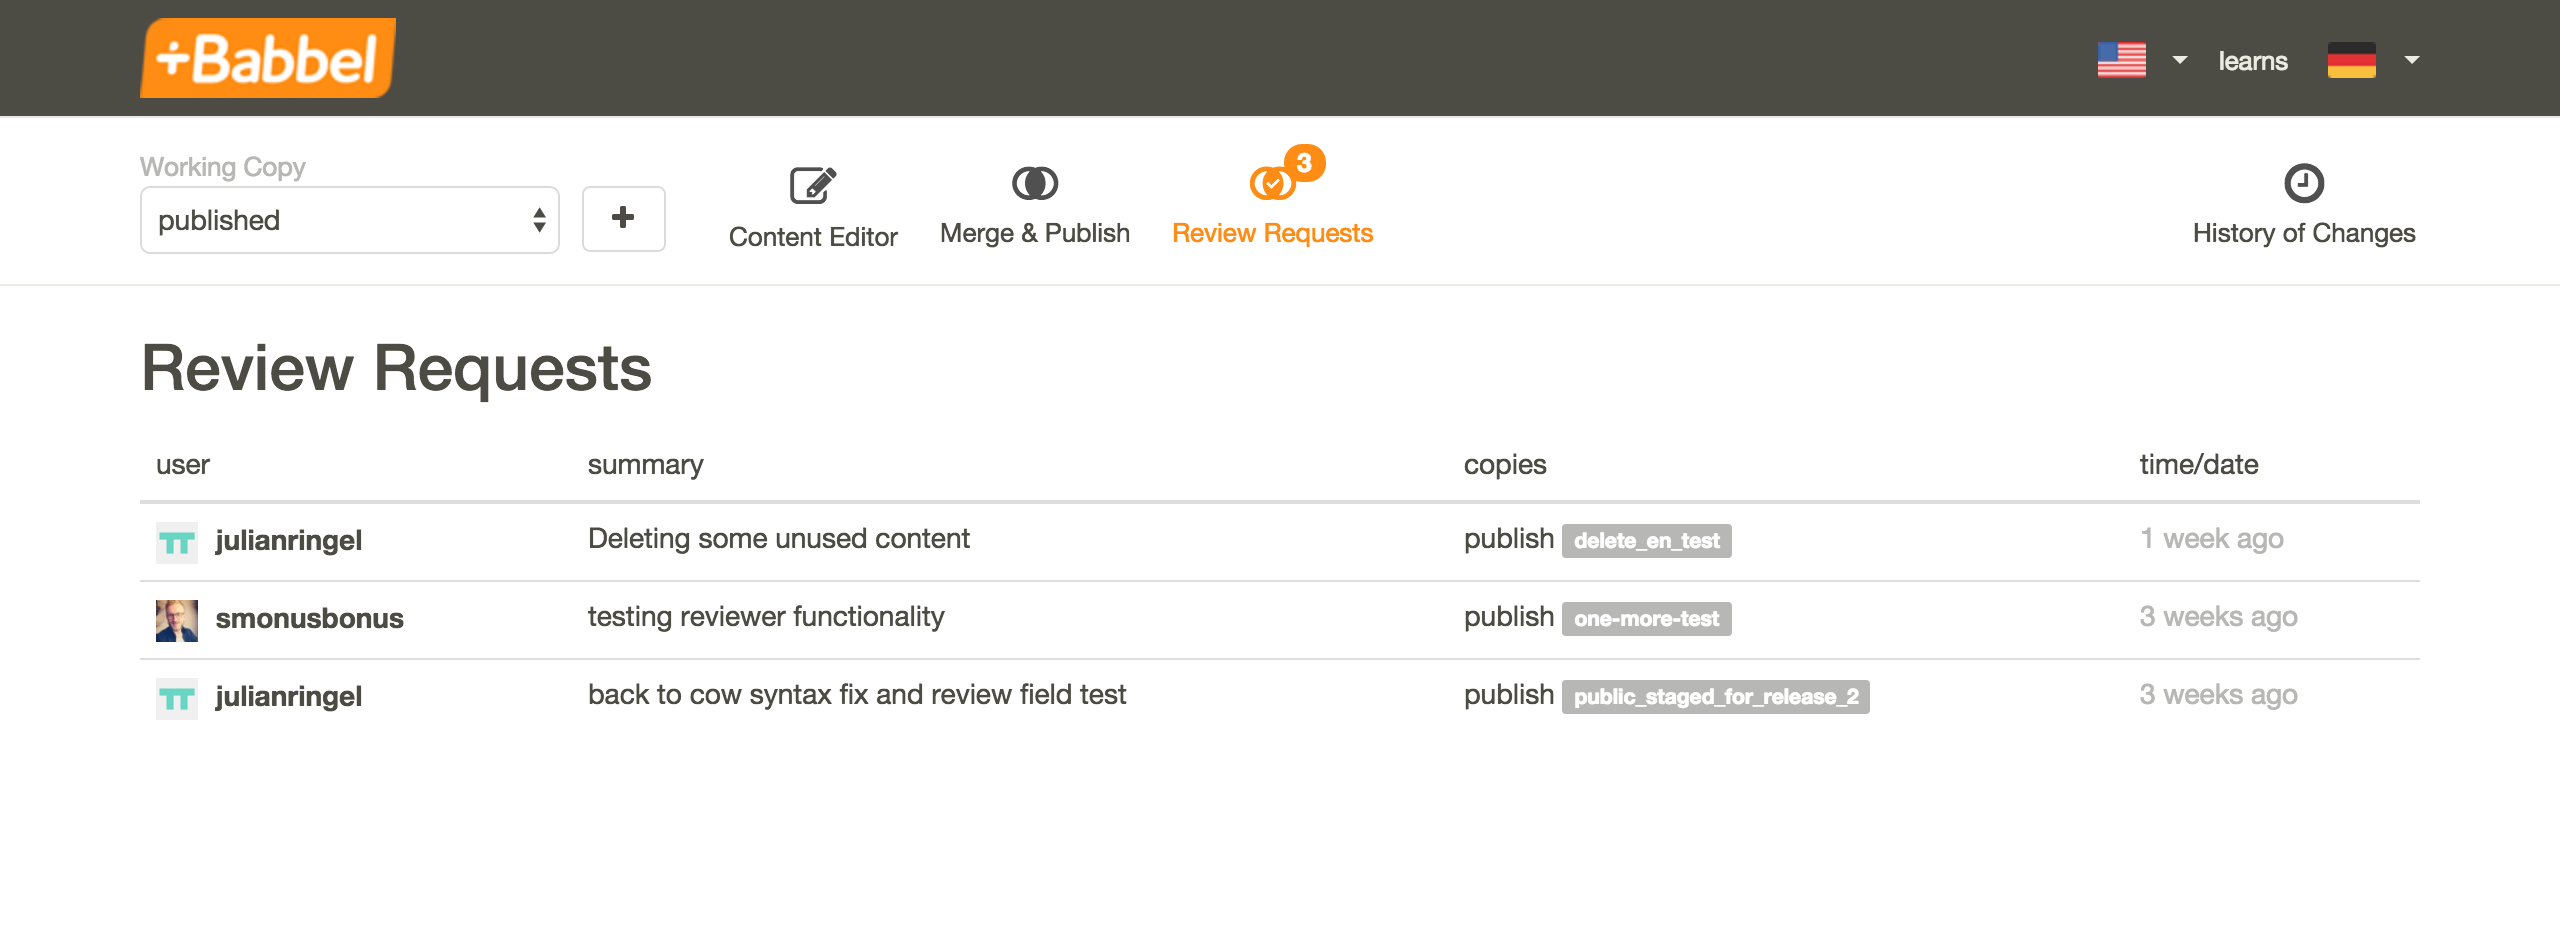
\includegraphics[width=\textwidth]{final-design/review-requests}}
 \caption{List of requests}
 \label{fig:review-requests}
\end{figure}

\begin{figure}[h!]
 \centering
 \fbox{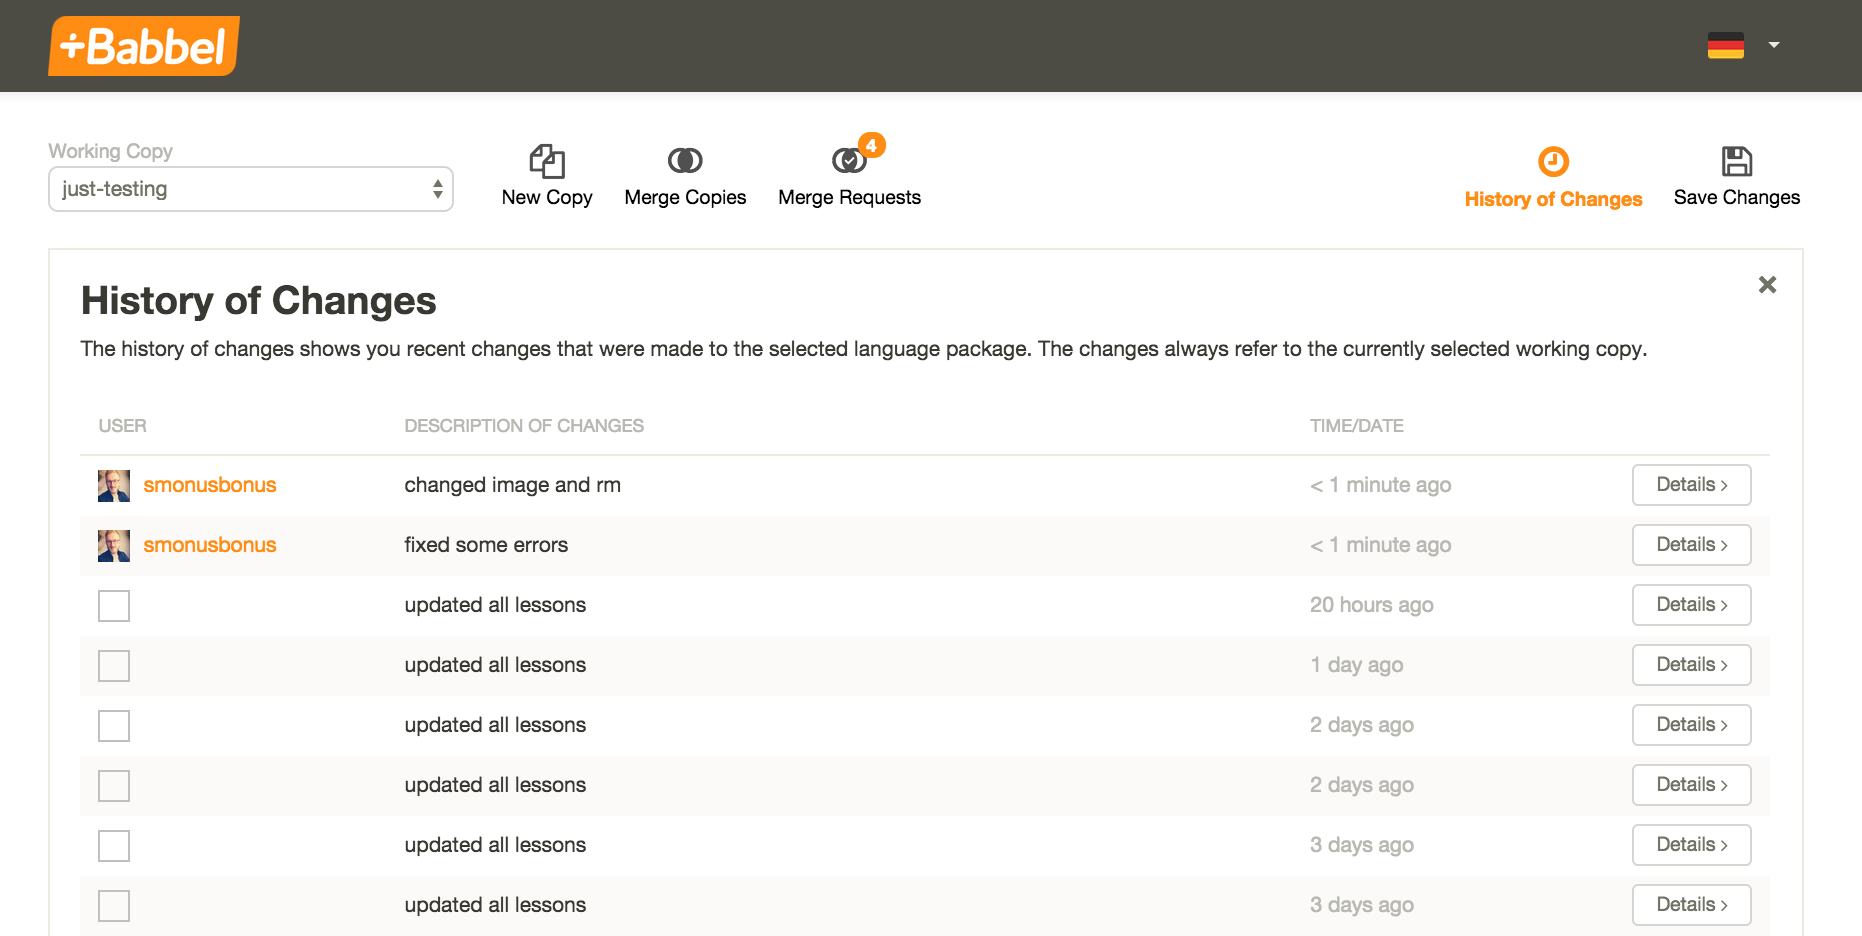
\includegraphics[width=\textwidth]{final-design/history}}
 \caption{History of changes}
 \label{fig:history-of-changes}
\end{figure}
